\documentclass[11pt,a4paper]{article}

\usepackage[utf8]{inputenc}
\usepackage[T1]{fontenc}
\usepackage{lmodern}
\usepackage{geometry}
\usepackage{xcolor}
\usepackage{enumitem}
\usepackage{listings}
\usepackage{booktabs}
\usepackage{array}
\usepackage{graphicx}
\geometry{margin=2.5cm}

\definecolor{codegray}{RGB}{245,245,245} 
\definecolor{darkblue}{RGB}{20,60,120}

\usepackage[
    colorlinks=true,
    linkcolor=darkblue,
    urlcolor=darkblue,
    citecolor=darkblue,
    breaklinks=true
]{hyperref}

\lstdefinestyle{codestyle}{
    backgroundcolor=\color{codegray},
    basicstyle=\ttfamily\small,
    breaklines=true,
    frame=single,
    columns=fullflexible,
    keepspaces=true,
    showstringspaces=false
}

\title{Demo Provenance-aware System}
\author{}
\date{}

\begin{document}

\maketitle



\section{Introduction}
Large Language Models (LLMs) are increasingly being used across various domains, including
text, image, and video generation, as well as data analysis and data manipulation.
Their ability to interpret user questions and produce fluent answers makes them suitable for Question Answering over structured data. However, when LLMs are applied to relational data, a generated answer is useful only if it can be related to the involved data source and represented in a form that can be inspected or checked.
This demo explores this setting through a modular system for Explainable Question Answering over tabular data. 
The system exposes a chat API compatible with OpenAI clients, while internally orchestrating several components commonly involved in LLM-based data interaction: row-level retrieval, model prompting, structured JSON generation and validation, query planning, deterministic execution, and provenance-based explanations.
Rather than acting as a database engine, the system is designed as a gateway for comparing different ways of combining LLMs with relational data. It supports multiple pipeline configurations, including retrieval-augmented generation, planner-based variants with deterministic execution, and an internal-knowledge baseline. This makes it possible to observe how different design choices affect the produced answer, the intermediate artifacts, and the available evidence.
 Users can submit natural language questions and inspect the generated structured output, retrieved records, planning artifacts, execution results, and provenance information. 



\section{Related Work}

\subsection{Retrieval-Augmented Generation}

Retrieval over tabular data requires different design choices from standard document retrieval. A common approach in RAG systems is to linearize tables into text and retrieve them as ordinary chunks. However, recent work has shown that this strategy may lose important tabular structure and provide only a partial view of the data, especially for questions requiring joins, filtering or aggregation. TableRAG ~\cite{yu2025tableragretrievalaugmentedgeneration} addresses this limitation by combining text retrieval with SQL-based execution over tabular components for heterogeneous document reasoning, showing the importance of preserving the distinction between textual and structured evidence. During an offline phase, the system extracts table contents, builds textual chunks for retrieval, stores table schemas, and also ingests the tables into a relational database. During online inference, it decomposes the user question, retrieves relevant chunks, maps retrieved table fragments back to their corresponding schemas, generates SQL when tabular reasoning is required, executes the SQL query over the relational database, and combines the execution result with retrieved textual evidence to generate the answer.

Our retrieval component follows a related motivation, but adapts it to relational CSV data. Instead of indexing arbitrary table chunks, we create one document for each table row. Each document contains a textual representation of the row, including the table name, primary-key values, column-value pairs, and selected foreign-key links to related rows. This row-level representation is designed to preserve enough relational structure for retrieval while remaining compatible with dense vector search. In addition, the document metadata stores the original table, row identifier, primary key, full row values, provenance row number when available, and linked-row information. The resulting documents are embedded with BGE-M3 and indexed with FAISS, enabling the system to retrieve candidate records that can later be used by the LLM.

Our retrieval design is also influenced by schema-aware approaches such as RAT-SQL~\cite{ratsql}. RAT-SQL addresses text-to-SQL parsing by making the structure of the database schema explicit: tables and columns are represented as graph nodes, while relations such as primary keys, foreign keys, and column-table membership are encoded as graph edges. This allows the model to reason not only over the textual form of the schema, but also over the relational connections that determine how tables and columns should be interpreted.

Although our system does not adopt RAT-SQL's neural parser, it follows a similar principle at the retrieval level. Each indexed document is not a plain textual chunk, but a structured representation of a relational row. In this way, relational information that would be hidden or lost in a naive text representation is made explicit before embedding and retrieval.


\subsection{Database Provenance}

\subsection{Databases and LLMs}
Recent work has investigated how database query-processing ideas can be adapted to interactions with Large Language Models. Satriani et al. introduce Galois ~\cite{EURECOM+8182}, a system that executes SQL queries over LLMs by treating the model as a data source and by defining LLM-aware logical and physical operators. In particular, Galois introduces LLMScan and Filter-LLMScan operators, which retrieve tuples from the model either without or with pushed-down selection conditions. Their work shows that complex data-oriented queries can benefit from being decomposed into operator-level plans, and that deciding whether conditions should be pushed into the LLM call involves a trade-off between cost and result quality.

Our demo system takes inspiration from this operator-oriented view, but adapts it to a different setting. In our planner-based pipelines, we introduce analogous LeafScan and FilterLeafScan steps. These steps are applied to the leaves of a generated tree plan and are used to query the LLM on smaller tasks, optionally with filter conditions pushed into the leaf. Unlike Galois, however, our system does not treat the LLM as the primary storage layer. The data source remains an explicit collection of relational tables, and the LLM is used as part of a pipeline involving retrieval, planning, structured generation, deterministic execution, and provenance explanation.

This distinction is central to our use of the idea. While Galois studies how SQL execution can be optimized when the LLM itself is queried as a data source, our system studies how LLM calls can be organized around a planner when answering questions over existing tabular data. 

\section{Architecture}

\subsection{System Overview}

The gateway is implemented as a FastAPI application in \texttt{gateway.py}. It
loads CSV files, maintains row-id indexes, manages a FAISS vector store,
calls Ollama models, validates JSON outputs, stores debug state, and exposes
OpenAI-compatible endpoints.

At a high level, a request follows these steps:

\begin{enumerate}[leftmargin=*]
    \item A client sends a chat-completion request to
    \texttt{/v1/chat/completions}.
    \item The gateway extracts the latest user message.
    \item The selected UI model id is mapped to an Ollama model name.
    \item The request is routed to one of the gateway modes:
    \begin{itemize}
        \item standard RAG;
        \item planner-first;
        \item planner-first explanation;
        \item internal-knowledge baseline.
    \end{itemize}
    \item The selected path performs retrieval, planning, model calls, and
    validation as required.
    \item The gateway returns an OpenAI-compatible chat-completion response.
    \item Debug information is stored for inspection through \texttt{/debug/ui}.
\end{enumerate}
\begin{figure}[h]
    \centering
    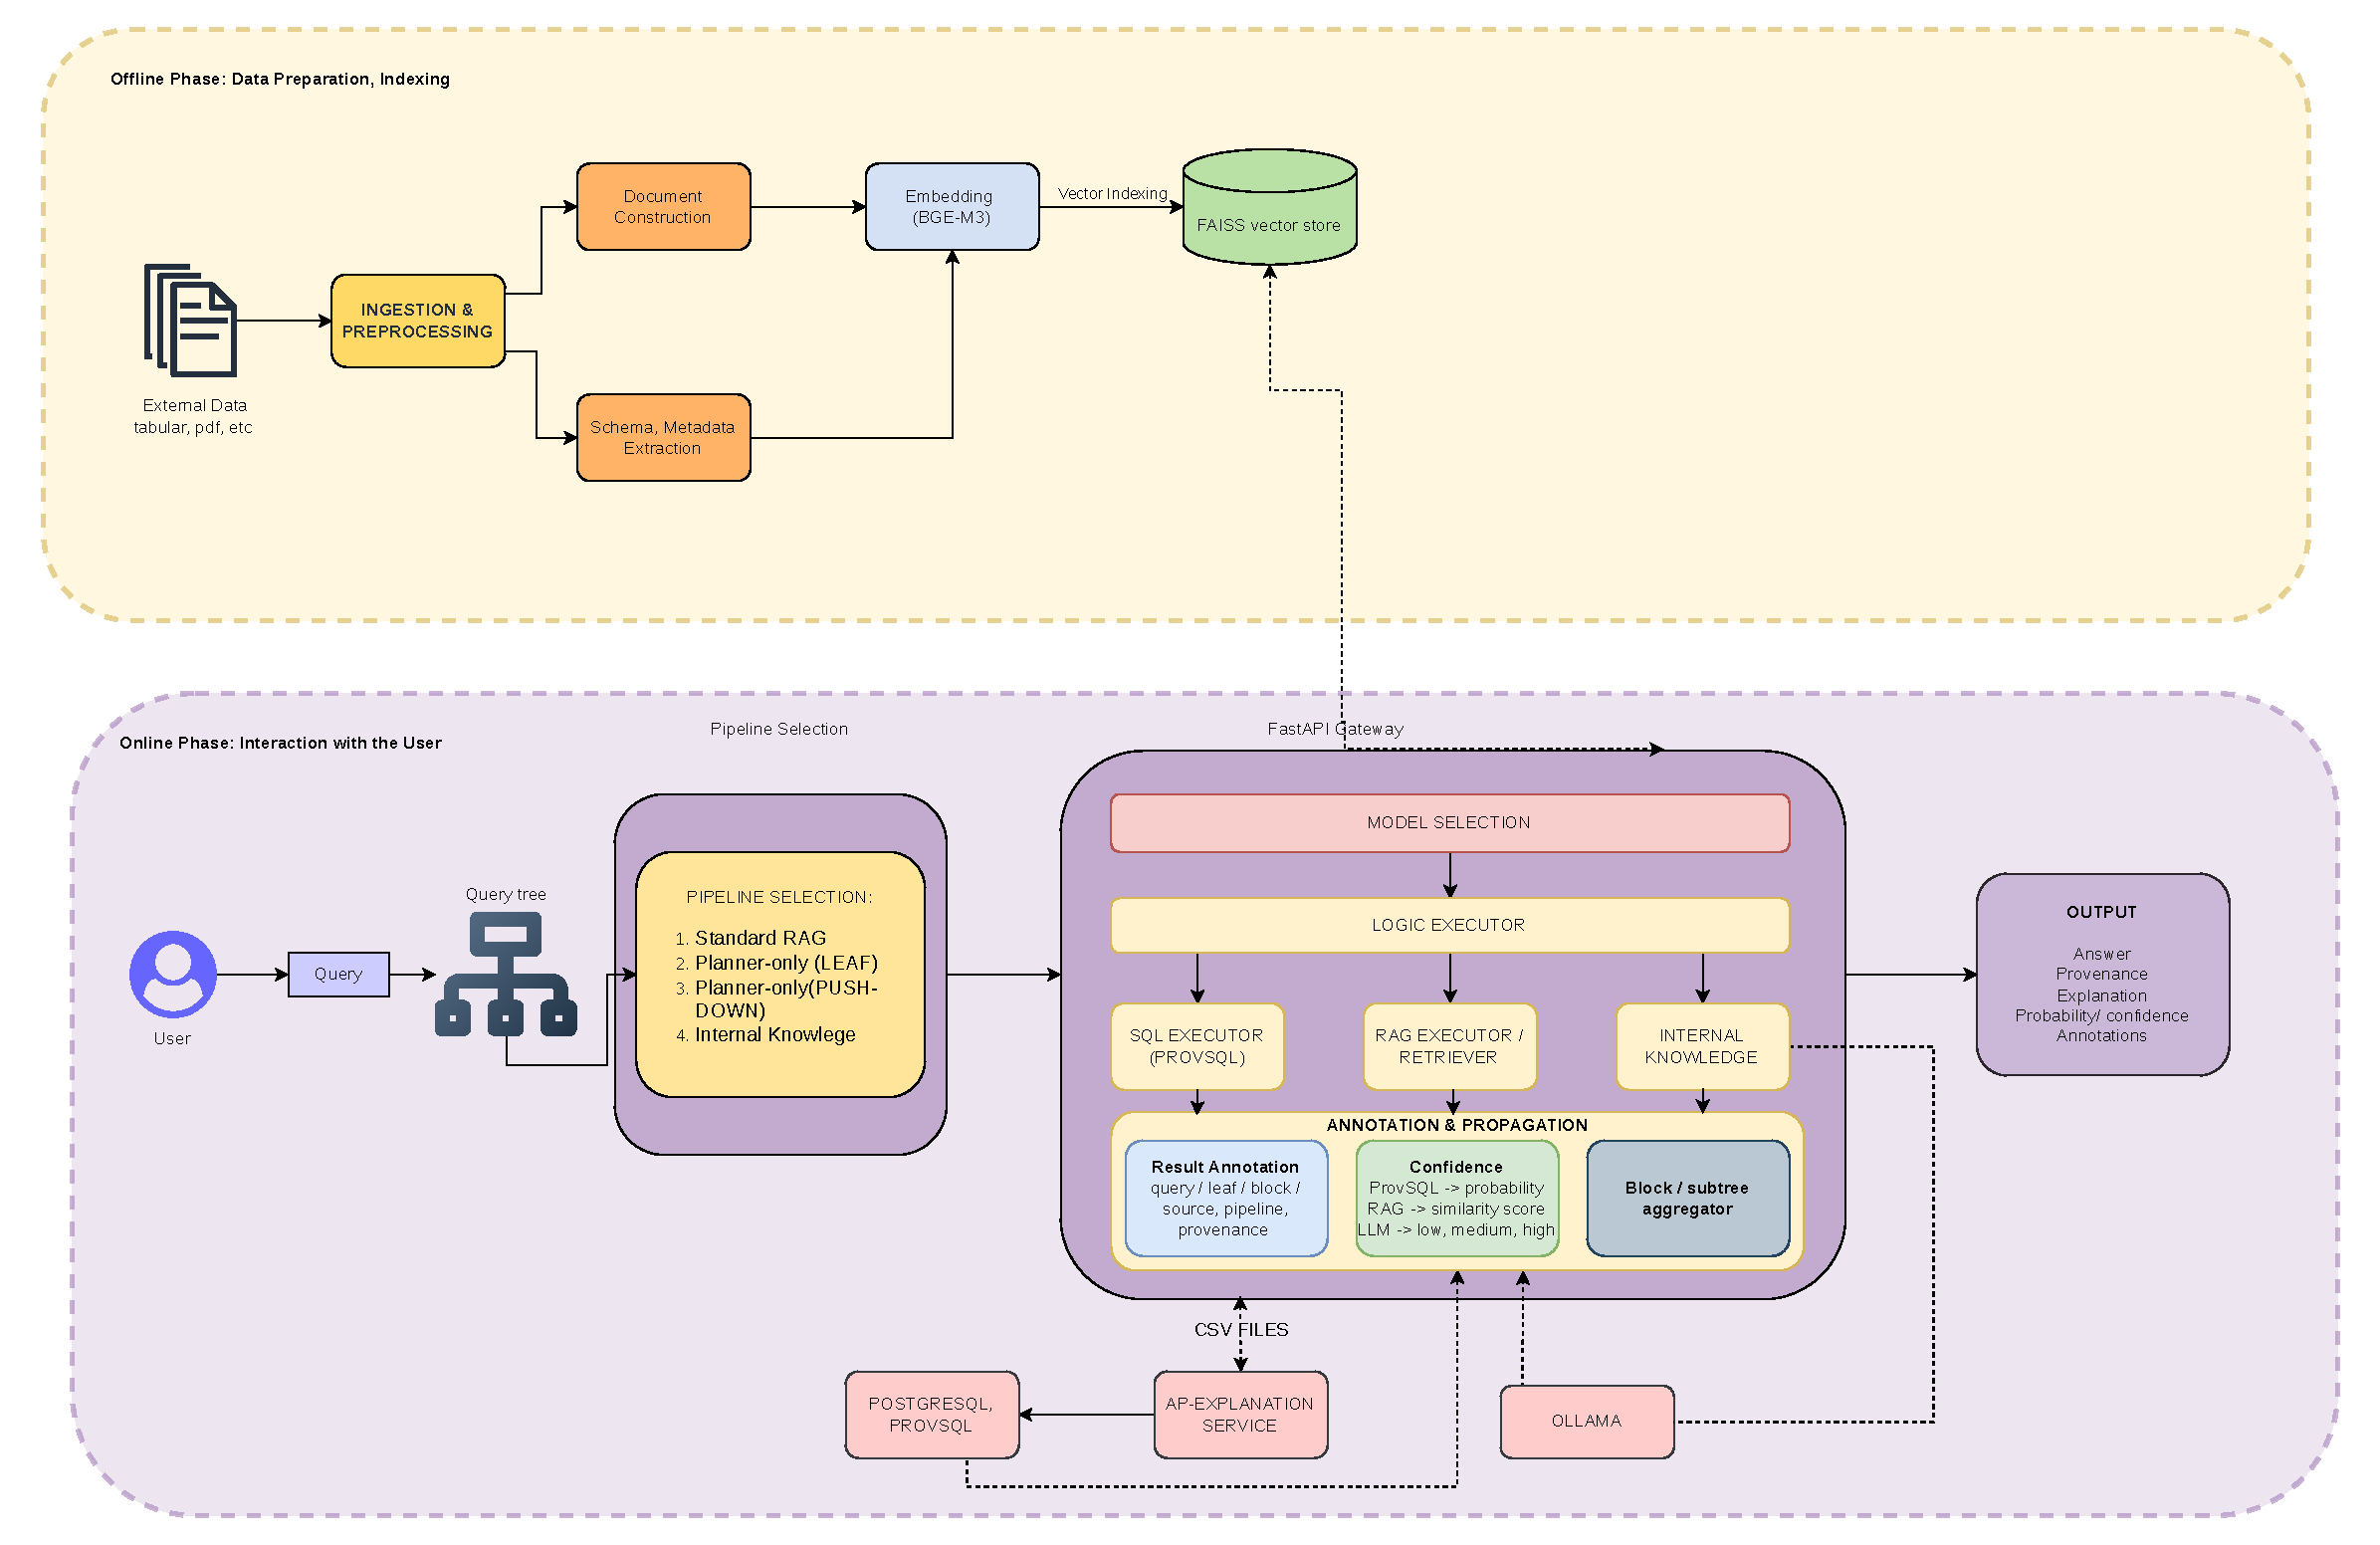
\includegraphics[width=1\textwidth]{architecture.pdf}
    \caption{Demo gateway architecture.}
    \label{fig:demo_gateway_architecture}
\end{figure}

\subsection{Model Routing}

The user interface shows model identifiers. These identifiers are
mapped to concrete Ollama models through environment variables:

\begin{lstlisting}[style=codestyle]
MODEL_ROUTING = {
    "base-llama3-8b": OLLAMA_MODEL_BASE,
    "best-ft-llama3-8b-nl": OLLAMA_MODEL_FT_NL,
    "best-ft-llama3-8b-sql": OLLAMA_MODEL_FT_SQL,
    "planner-first": OLLAMA_MODEL_PLANNER_FIRST,
    "planner-first-explanation": OLLAMA_MODEL_PLANNER_FIRST_EXPLANATION,
    "internal-knowledge": OLLAMA_MODEL_INTERNAL_KNOWLEDGE,
}
\end{lstlisting}

Only the logical identifiers are exposed through \texttt{/v1/models}. This keeps
the UI stable when local model names or Ollama tags change.

\subsection{Row-Level Data Layer}

The data layer is built from CSV files. Each table contains
a row-number column such as \texttt{nation\_rownum}; this value becomes the local
row identifier. When CSVs are loaded, the gateway builds:

\begin{itemize}[leftmargin=*]
    \item an in-memory table cache;
    \item a per-table mapping from row id to row position;
    \item a global row-id index for provenance resolution.
\end{itemize}


\subsection{FAISS Retrieval Layer}

The retrieval layer is managed by \texttt{FaissIndexManager}. The current row
index is built from one document per source row. Documents are embedded with
BGE-M3 in the row-index workflow and store structured metadata including table
name and row identifier. After FAISS returns nearest documents, the gateway uses
the metadata to reconstruct exact CSV rows from the in-memory cache.

The iterative retrieval function starts with \texttt{RETRIEVER\_K} neighbors and
increases the requested depth by \texttt{RETRIEVER\_K} at each iteration. It
stops when no new rows are added or when
\texttt{MAX\_ITERATIVE\_RETRIEVALS} is reached. Duplicate row ids are ignored,
unresolvable row ids are skipped, and \texttt{MAX\_TABLES} limits the number of
tables represented in the context.

\subsection{Standard RAG Path}

In the standard path, the latest user message is treated as a natural-language
question. The gateway retrieves row context with the question itself as the
retrieval query, serializes retrieved rows into prompt text, and asks the model
to return a JSON array:

\begin{lstlisting}[style=codestyle]
[
  {
    "result": {...},
    "provenance": [["table_1"], ["table_2", "table_3"]]
  }
]
\end{lstlisting}

This path is useful as a baseline, but it leaves most reasoning to the model:
answer construction, row selection, and provenance construction happen in a
single generation step.

\subsection{Planner-First Path}

The planner-first path is selected with the model id \texttt{planner-first}. The
input is interpreted as SQL. The gateway calls \texttt{build\_query\_plan}, which
returns a \texttt{QueryPlan} containing:

\begin{itemize}[leftmargin=*]
    \item the original SQL and query type;
    \item one \texttt{LeafExtractionTask} per table;
    \item join specifications;
    \item post-operations for relational work after leaf extraction.
\end{itemize}

For each leaf task, the gateway builds a compact retrieval query such as:

\begin{lstlisting}[style=codestyle]
table: nation | columns: n_name, n_regionkey
\end{lstlisting}

It then retrieves candidate rows, builds a strict leaf prompt, calls the model,
and validates the output. The response contains the full plan and the leaf
outputs, including retrieved context, prompt, raw model output, parsed rows, and
validation status.

\subsection{Leaf Output Contract}

Each leaf output must be a JSON array. Every item must contain exactly
\texttt{row\_id} and \texttt{values}:

\begin{lstlisting}[style=codestyle]
[
  {
    "row_id": "nation_2",
    "values": {
      "nation_rownum": "nation_2",
      "n_name": "ARGENTINA",
      "__rid__": "nation_2"
    }
  }
]
\end{lstlisting}

Validation is intentionally strict. The root must be an array, each item must be
an object, \texttt{row\_id} must be a string, row ids must not be duplicated, and
\texttt{values} must exactly match the corresponding retrieved row. If
\texttt{\_\_rid\_\_} is present inside \texttt{values}, it must equal
\texttt{row\_id}. The parser also keeps individually valid items from otherwise
invalid outputs, which supports partial evaluation.

\subsection{Planner-First Explanation Path}

The model id \texttt{planner-first-explanation} runs the planner-first pipeline
and then sends the extracted leaf rows to an external explanation service. The
pipeline:

\begin{enumerate}[leftmargin=*]
    \item runs planner-first extraction;
    \item converts leaf outputs into one CSV file per table;
    \item writes the CSV files to a shared bucket directory;
    \item builds an AP explanation payload;
    \item sends the job to the AP explanation service;
    \item polls for completion when the service returns an asynchronous task id;
    \item renders the result as markdown for the UI.
\end{enumerate}

This path connects the language-model gateway to a provenance-aware backend
using PostgreSQL with ProvSQL support.

\subsubsection{Provenance Explanation Endpoint}

The gateway also exposes a provenance explanation workflow for standard JSON
answers. It parses an answer with \texttt{result} and \texttt{provenance}, checks
the witness-set structure, resolves row identifiers through the global row-id
index, and can call an explanation model with the relevant schema subset and
source rows. The workflow detects empty witness sets, duplicate row ids inside a
witness set, unknown row ids, and duplicate witness sets.

\bibliographystyle{plain}
\bibliography{bibfile}

\end{document}
